\documentclass[psamsfonts]{amsart}

%-------Packages---------
\usepackage{amssymb,amsfonts}
\usepackage[all,arc]{xy}
\usepackage{enumerate}
\usepackage{mathrsfs}
\usepackage{subcaption}
\usepackage{graphicx}
\usepackage{caption}

%--------Theorem Environments--------
%theoremstyle{plain} --- default
\newtheorem{thm}{Theorem}[section]
\newtheorem{cor}[thm]{Corollary}
\newtheorem{prop}[thm]{Proposition}
\newtheorem{lem}[thm]{Lemma}
\newtheorem{conj}[thm]{Conjecture}
\newtheorem{quest}[thm]{Question}

\theoremstyle{definition}
\newtheorem{defn}[thm]{Definition}
\newtheorem{defns}[thm]{Definitions}
\newtheorem{con}[thm]{Construction}
\newtheorem{exmp}[thm]{Example}
\newtheorem{exmps}[thm]{Examples}
\newtheorem{notn}[thm]{Notation}
\newtheorem{notns}[thm]{Notations}
\newtheorem{addm}[thm]{Addendum}
\newtheorem{exer}[thm]{Exercise}

\theoremstyle{remark}
\newtheorem{rem}[thm]{Remark}
\newtheorem{rems}[thm]{Remarks}
\newtheorem{warn}[thm]{Warning}
\newtheorem{sch}[thm]{Scholium}

\makeatletter
\let\c@equation\c@thm
\makeatother
\numberwithin{equation}{section}

\bibliographystyle{plain}

%--------Meta Data: Fill in your info------
\title{Problem Set 1 \\ STAT 221}

\author{Won I. Lee}

%\date{July 30, 2016}


\begin{document}
	
\maketitle

\section{Implement Gradient Descent}

In this section, we investigate the performance of gradient descent-based algorithms for minimizing scalar functions of vector arguments. In particular, we consider the following functions: 1) the negative Gaussian function:

$$f(x) = -\frac{1}{\sqrt{(2\pi)^n |\Sigma|}} \exp\left[ -\frac{1}{2}(x-u)^T\Sigma^{-1}(x-u) \right]$$

and 2) the quadratic bowl function:

$$f(x) = \frac{1}{2}x^TAx - x^Tb$$

\subsection{Initialization and Hyperparameters} We first explore the batch gradient descent algorithm. For loss function $f(x)$, the gradient descent algorithm performs:

$$x = x - \eta \nabla f(x)$$

where $\eta$ is the step size. These iterations continue until a convergence criterion is met, i.e. $|f(x) - f(\tilde{x})| < \epsilon$, where $x, \tilde{x}$ are successive iterations. We investigate the dependence of this algorithm on the initialization of the algorithm as well as its hyperparameters, namely the step size $\eta$ and the convergence criterion $\epsilon$. Throughout the experiments, we fix the following parameters of the functions:

$$u = (10, 10)$$
$$\Sigma = \begin{pmatrix} 1000 & 0 \\ 0 & 1000\end{pmatrix}$$
$$A = \begin{pmatrix} 10 & 5 \\ 5 & 10\end{pmatrix}$$
$$b = (400, 400)$$

First, we note that such a large variance in the negative Gaussian density yields very small objective function values (as they are scaled by the reciprocal of the determinant of $\Sigma$), as well as small gradient updates. Thus, we consider only large step sizes that will yield noticeable increments in the values of $x$; otherwise, no learning is achieved. Similarly, we only consider very small $\epsilon$ for the same reasons.

The results are shown in {\bf Figure 1} for the negative Gaussian function, where the $z$-axis is the squared distance. We have used step sizes of $10^5, 10^6, \dots, 10^10$ and convergence criteria of $10^{-10}, 10^{-11}, \dots, 10^{-20}$. The plots reveal two major points. First, for any choice of initialization and step size used in the experiments, gradient descent does not converge to a suitable solution until $\epsilon$, the convergence criterion, is sufficient small. As the plots demonstrate, we require $\epsilon \approx 10^{-15}$ or $\log(\epsilon) \approx -35$ before the squared error falls to negligible values. Second, the step size must bee sufficiently large before convergence is achieved, in the same vein as the convergence criterion. Even for suitable $\epsilon$ values, a relatively small step size (i.e. $10^5$) does not yield approximate convergence to the correct solution. Indeed, for most cases, we require a step size of $\eta \approx 10^7$ before the suared loss becomes negligible. As discussed above, these issues are germane to the negative Gaussian function, due to the large determinant value effectively annihilating the step sizes unless sufficiently large.

On the other hand, the quadratic bowl function does not have such issues, and using large step sizes generally yields divergence. Indeed, even using $\eta = 1$ leads to diverging estimates for $\epsilon \approx 10^{-15}$. Thus, for this case we consider step sizes of $10^{-1}, 10^{-2}, \dots, 10^{-5}$ and similarly convergence criteria of $10^{-10}, 10^{-11}, \dots, 10^{-20}$. Results as shown in {\bf Figure 2} demonstrate a very similar behavior for the quadratic bowl function; the convergence criterion $\epsilon$ must be suitably small for convergence to the correct values. In this case, however, if the step size $\eta$ is too small, then no $\epsilon$ used in our experiments can yield convergence, unlike the case of the negative Gaussian, in which a suitably small $\epsilon$ would yield convergence in all step sizes. We must have a large enough step size (in this case $\eta \approx 0.01$) for convergence in this example.

\begin{figure}
	\centering
	\begin{subfigure}[b]{0.45\textwidth}
	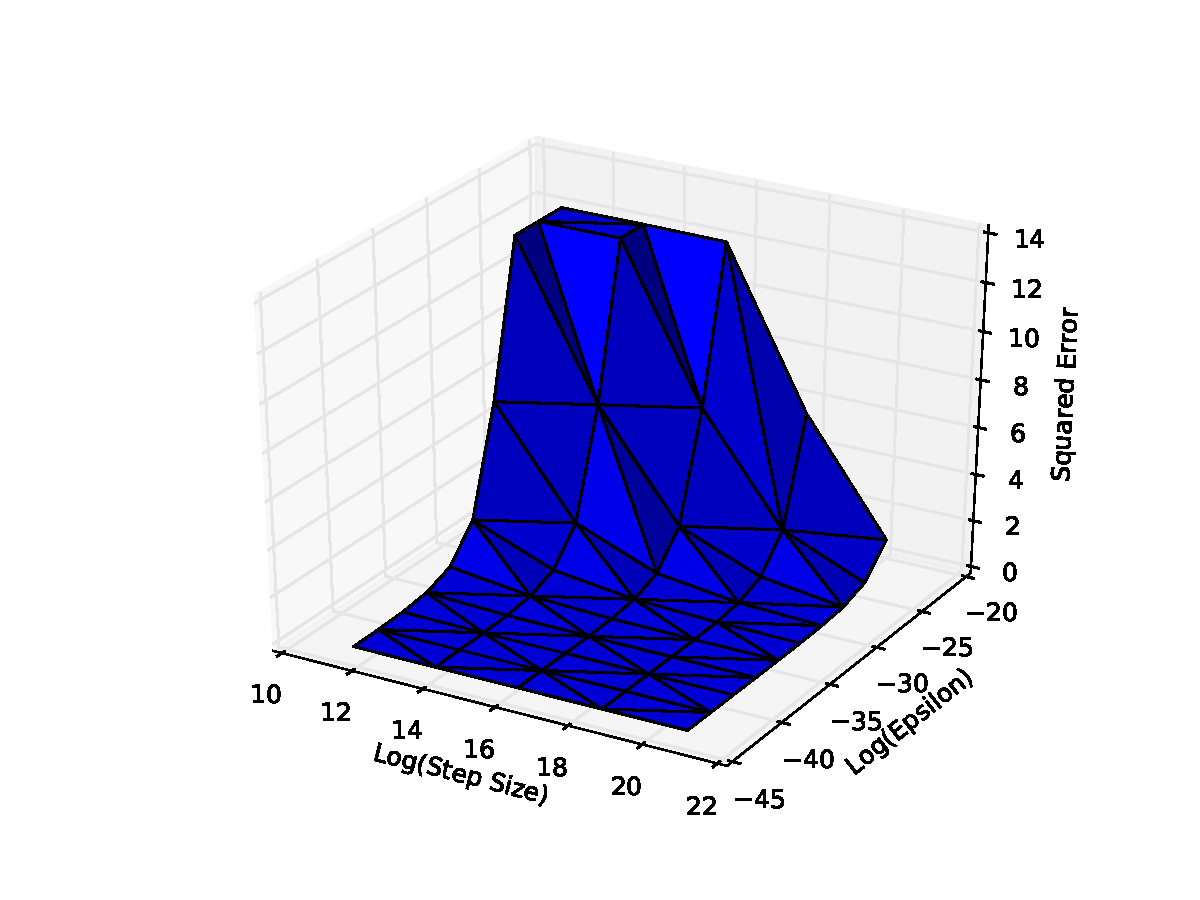
\includegraphics[width=\textwidth]{hw1_1-1_0.pdf}
	\caption{(1,1)}
	\end{subfigure}
\begin{subfigure}[b]{0.45\textwidth}
	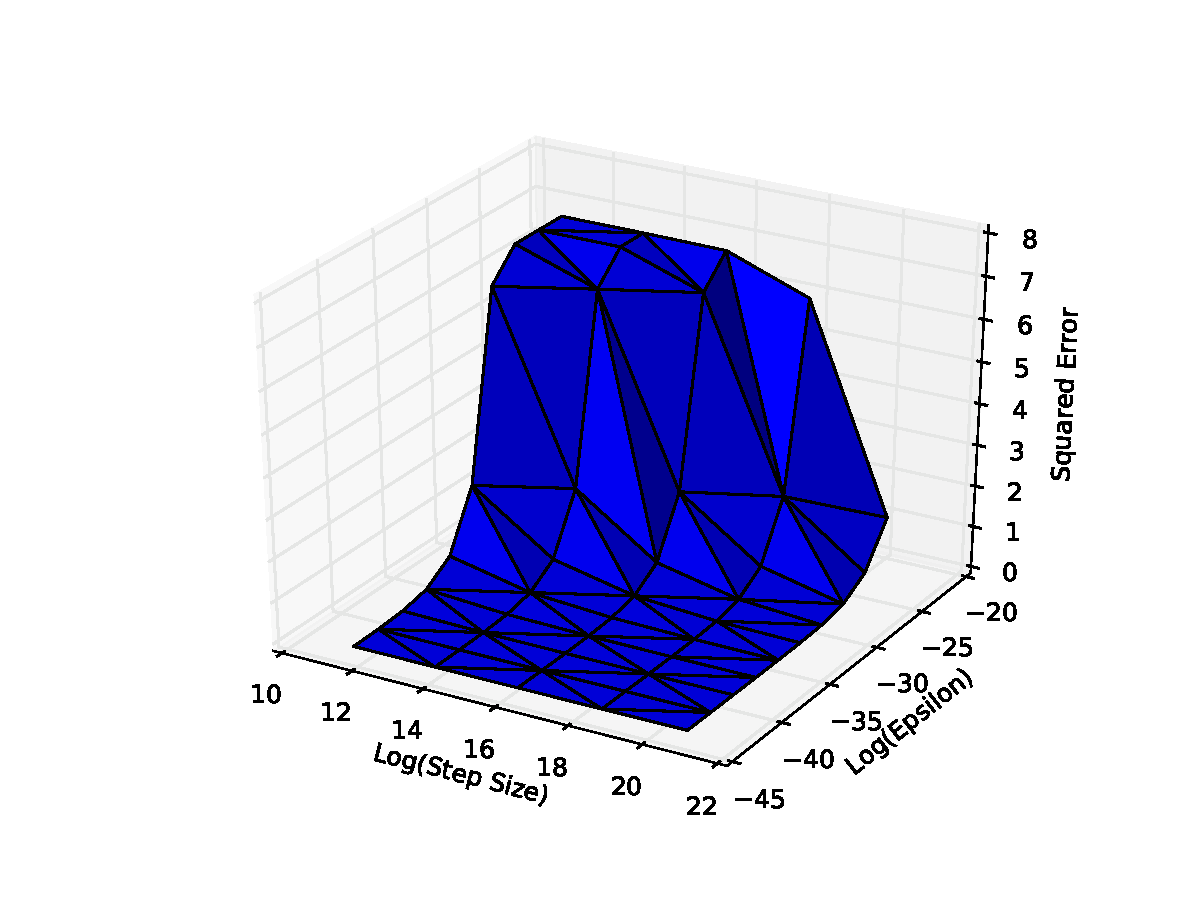
\includegraphics[width=\textwidth]{hw1_1-1_1.pdf}
	\caption{(5,5)}
\end{subfigure}
\begin{subfigure}[b]{0.45\textwidth}
	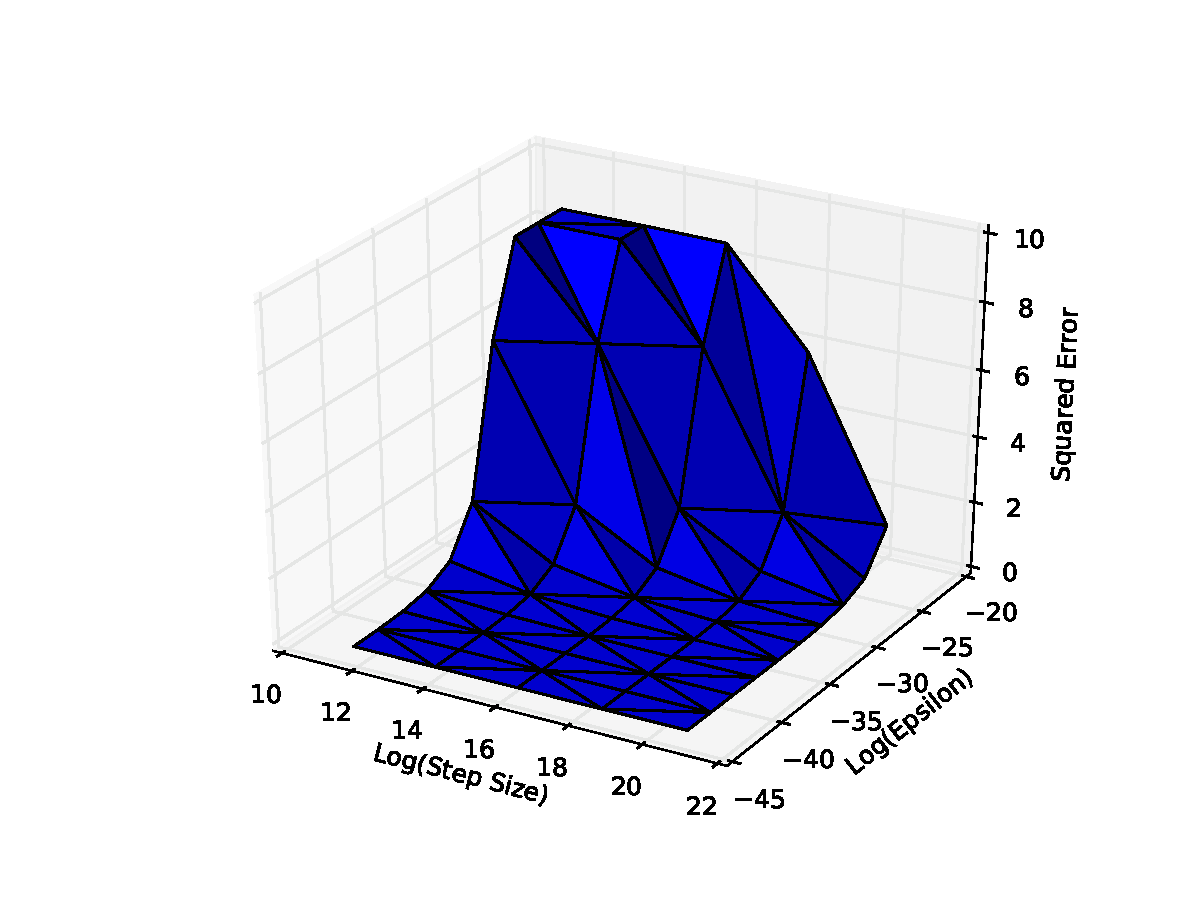
\includegraphics[width=\textwidth]{hw1_1-1_2.pdf}
	\caption{(1,9)}
	\end{subfigure}
	\begin{subfigure}[b]{0.45\textwidth}
		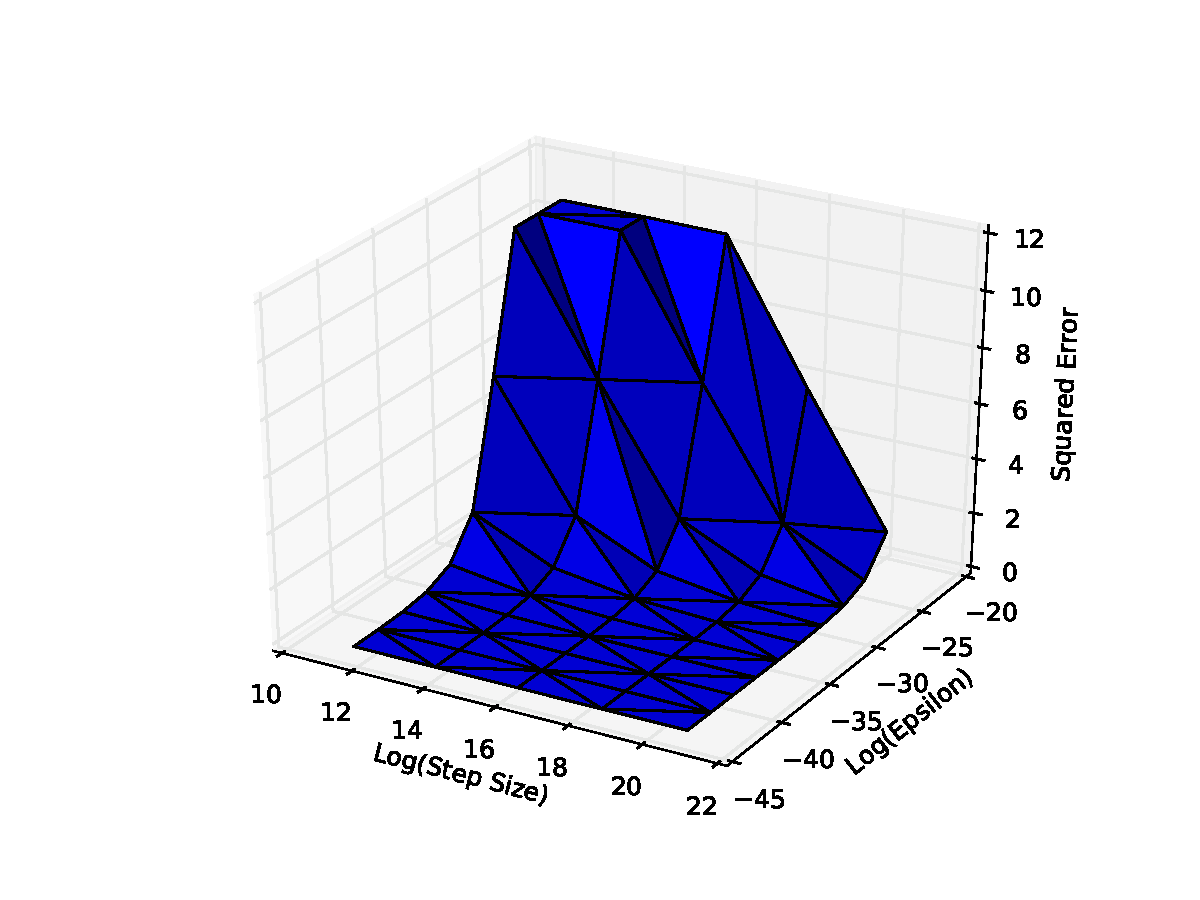
\includegraphics[width=\textwidth]{hw1_1-1_3.pdf}
		\caption{(20,15)}
		\end{subfigure}
\caption{Squared distance to correct solution $u$ using the negative Gaussian function for various starting points, step sizes, and convergence criteria. The labels on the plots are the starting points.}
\end{figure}

\begin{figure}
	\centering
	\begin{subfigure}[b]{0.45\textwidth}
		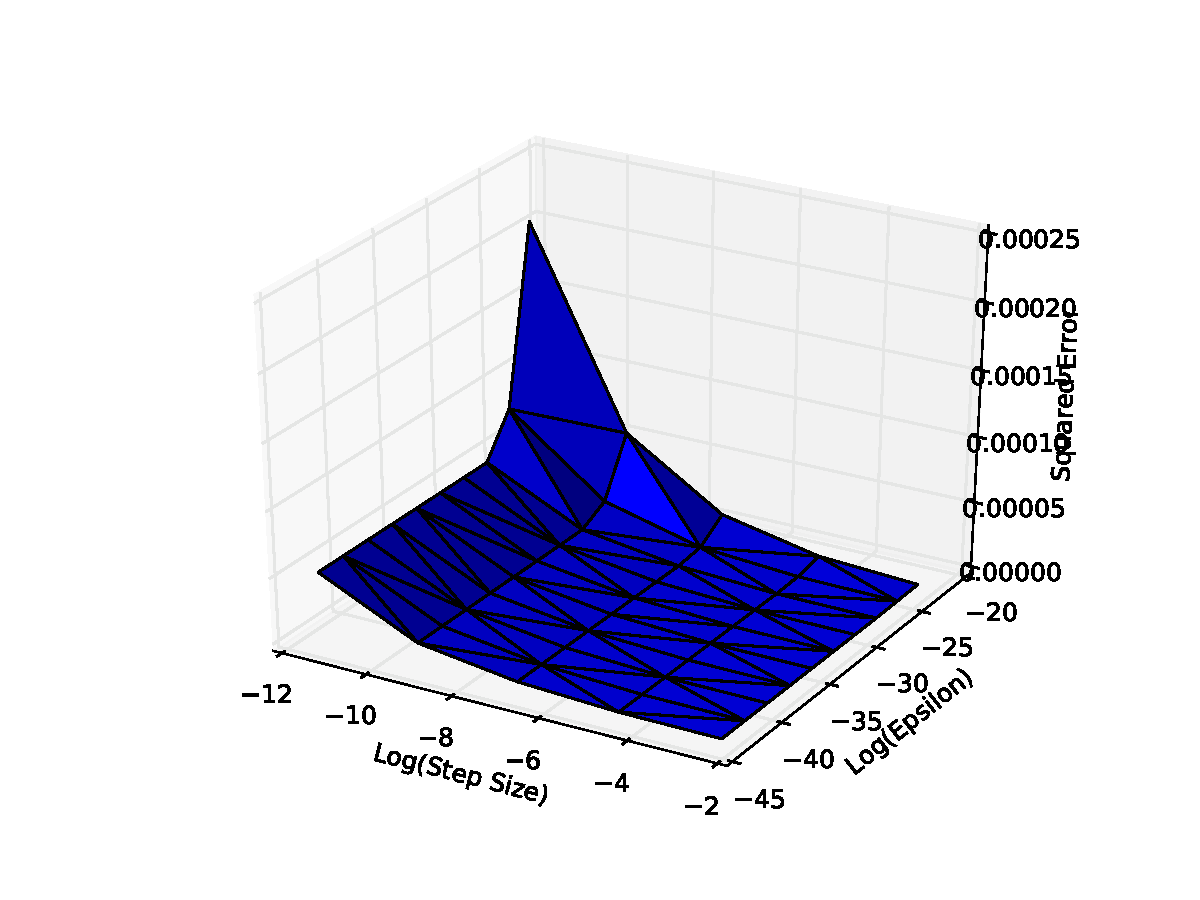
\includegraphics[width=\textwidth]{hw1_1-2_0.pdf}
		\caption{(1,1)}
	\end{subfigure}
	\begin{subfigure}[b]{0.45\textwidth}
		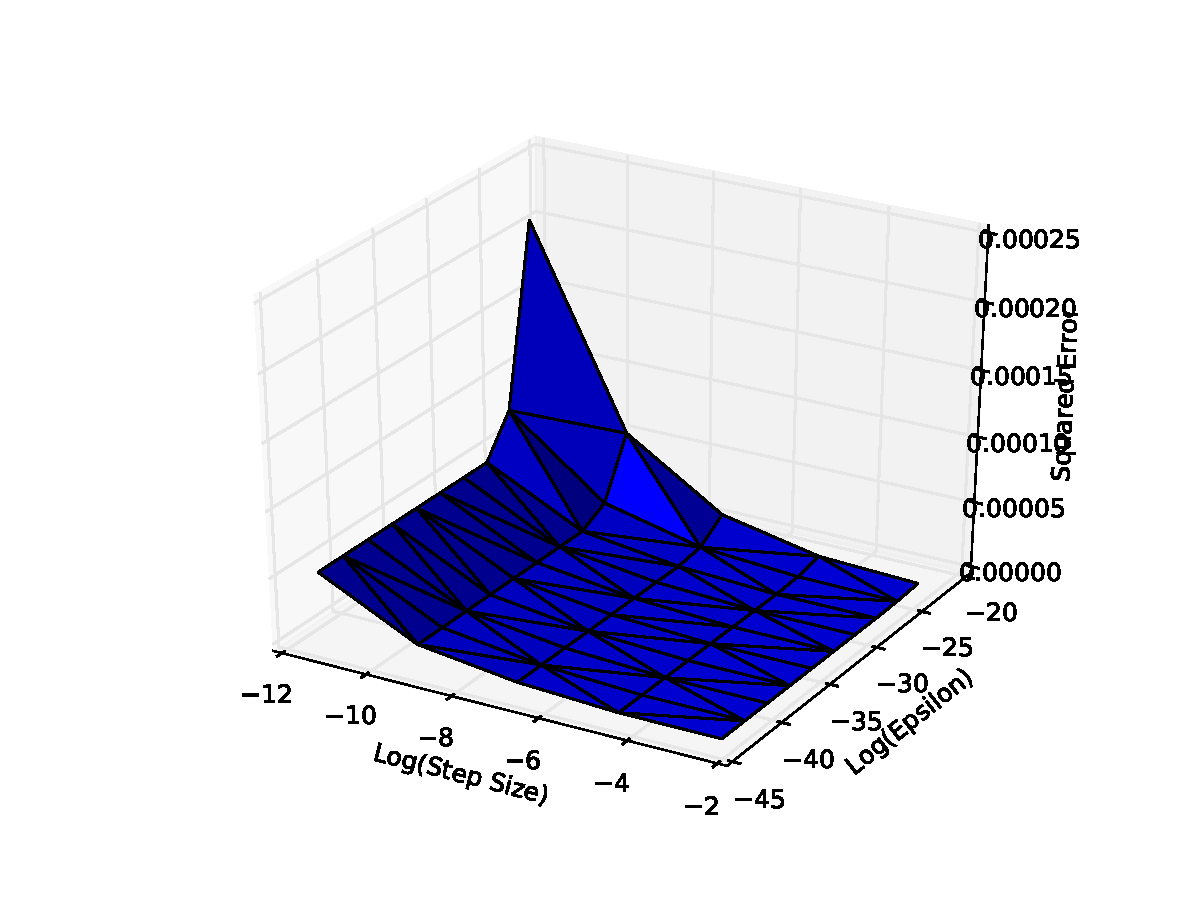
\includegraphics[width=\textwidth]{hw1_1-2_1.pdf}
		\caption{(5,5)}
	\end{subfigure}
	\begin{subfigure}[b]{0.45\textwidth}
		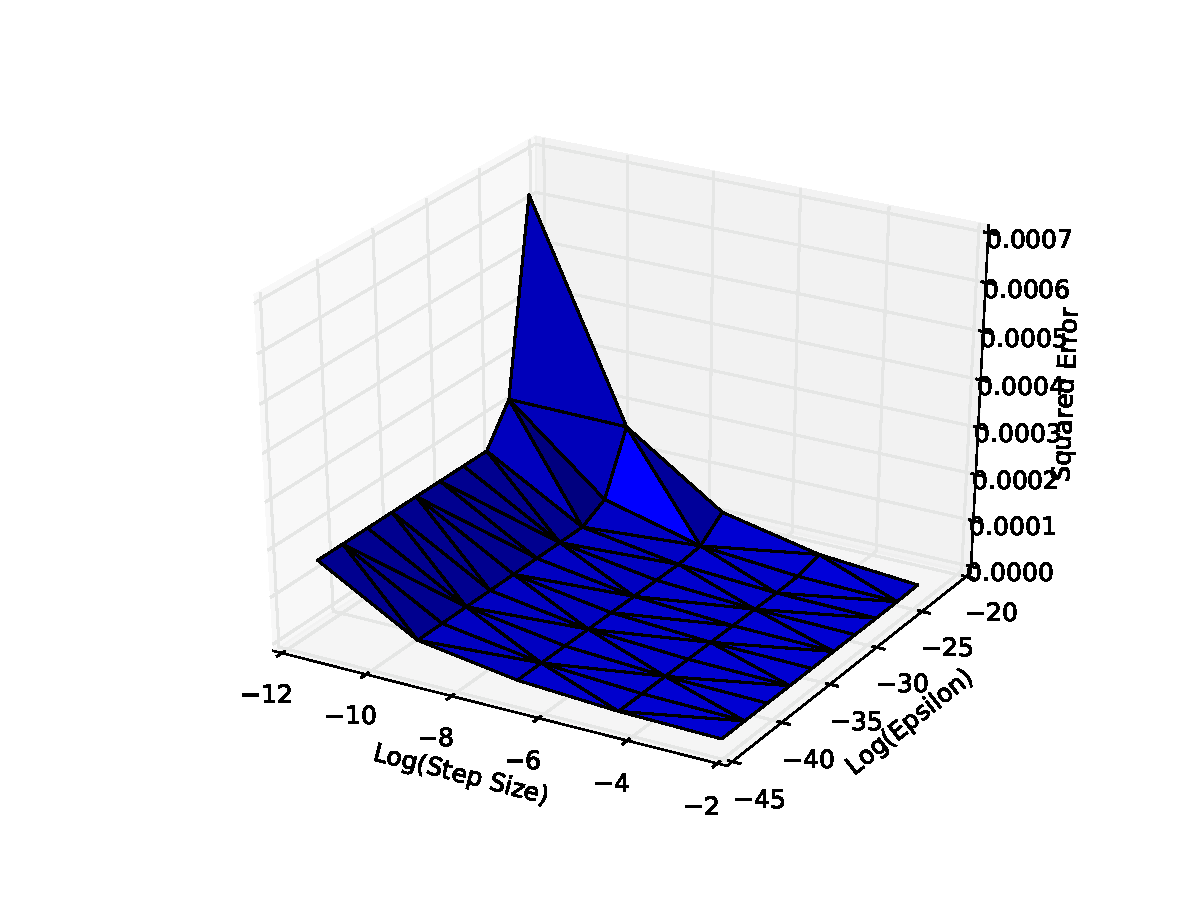
\includegraphics[width=\textwidth]{hw1_1-2_2.pdf}
		\caption{(1,9)}
	\end{subfigure}
	\begin{subfigure}[b]{0.45\textwidth}
		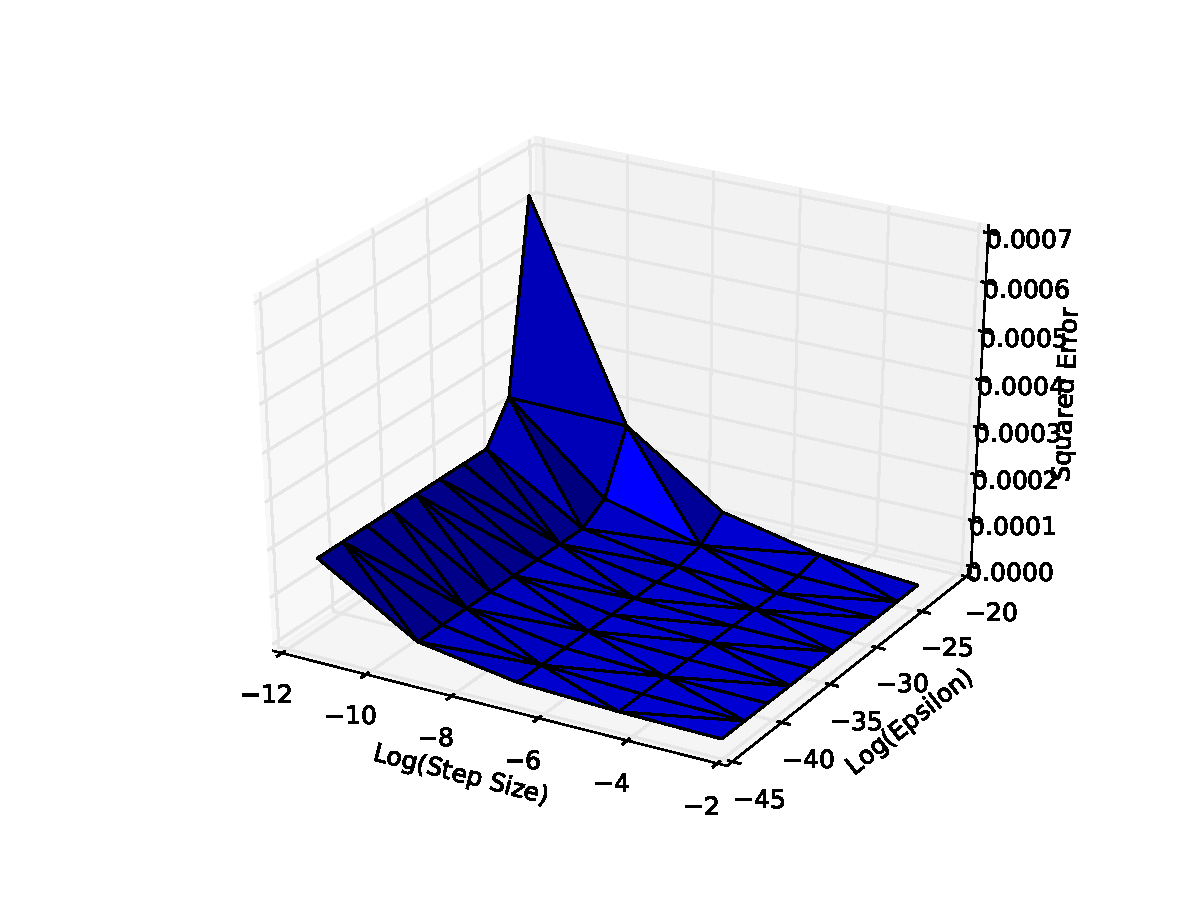
\includegraphics[width=\textwidth]{hw1_1-2_3.pdf}
		\caption{(20,15)}
	\end{subfigure}
	\caption{Squared distance to correct solution $u$ using the quadratic bowl function for various starting points, step sizes, and convergence criteria. The labels on the plots are the starting points.}
\end{figure}
	

\subsection{Comparison to Finite Differences} We compare the exact gradients obtained to finite difference approximations of the gradient using a central difference method:

$$\frac{\partial f(x)}{\partial x_i} \approx \frac{f(x + \delta e_i) - f(x - \delta e_i)}{2\delta}$$

where $\delta$ is the difference size and $e_i$ is a unit vector in the $i^{th}$ coordinate. We consider a number of different $\delta$ and compare the squared error between the true gradient and the finite approximation to the gradient. Namely, we compute the finite difference for $\delta = 1, 0.1, \dots, 10^{-4}$ and consider the points given in Figures 1 and 2. The result is given in {\bf Figure 3}, where we see that even for a step size of $\delta = 1$, we obtain a squared error of approximately $10^{-13}$ for the negative Gaussian and 0 for the quadratic bowl function (since it has a linear derivative). The nonzero squared error for smaller difference sizes for the quadratic bowl function is postulated to be due to numerical error, but even these are negligible. This demonstrates that for simple functions such as the two considered here, the finite difference gradient can be a cheap yet accurate approximation to the actual gradient.

\begin{figure}
\begin{subfigure}[b]{0.45\textwidth}
	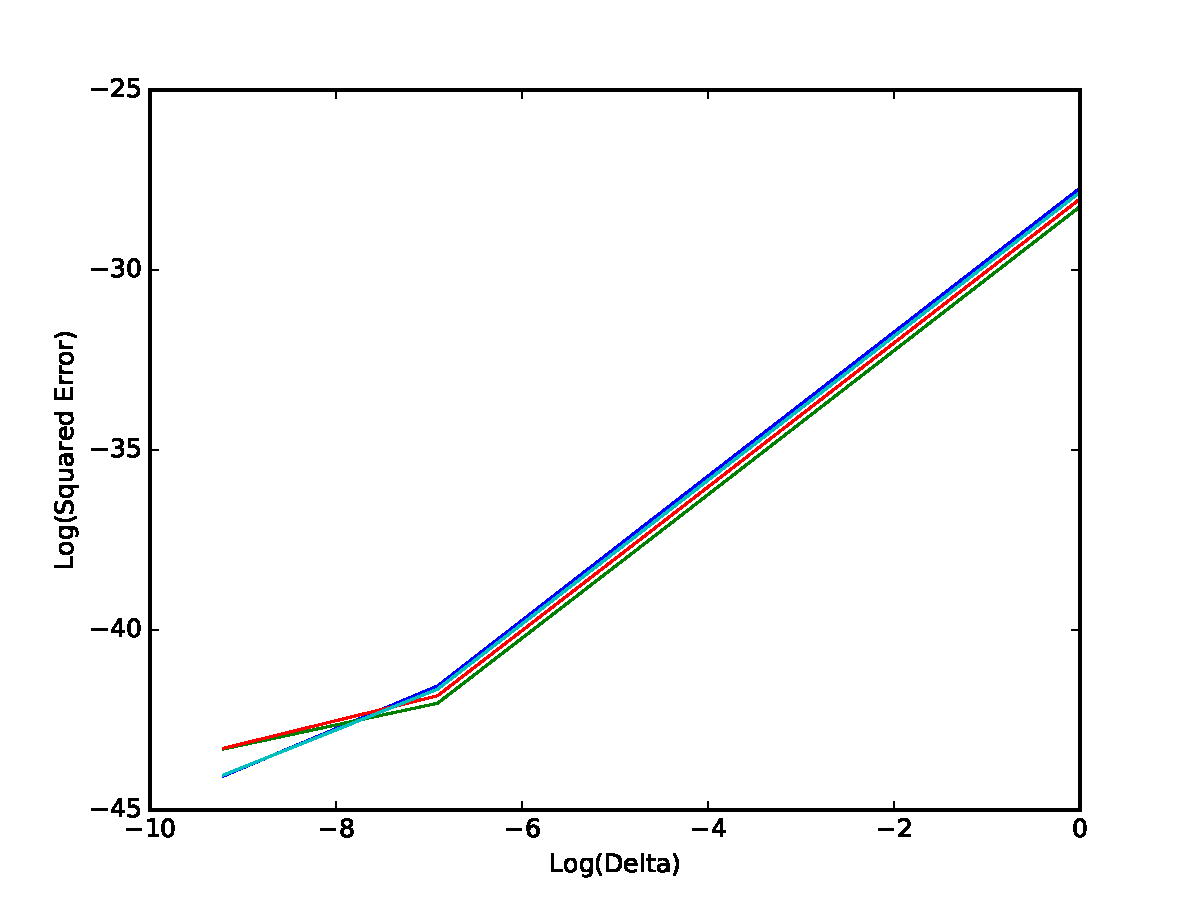
\includegraphics[width=\textwidth]{hw1_1-2a.pdf}
	\caption{Negative Gaussian}
\end{subfigure}
\begin{subfigure}[b]{0.45\textwidth}
	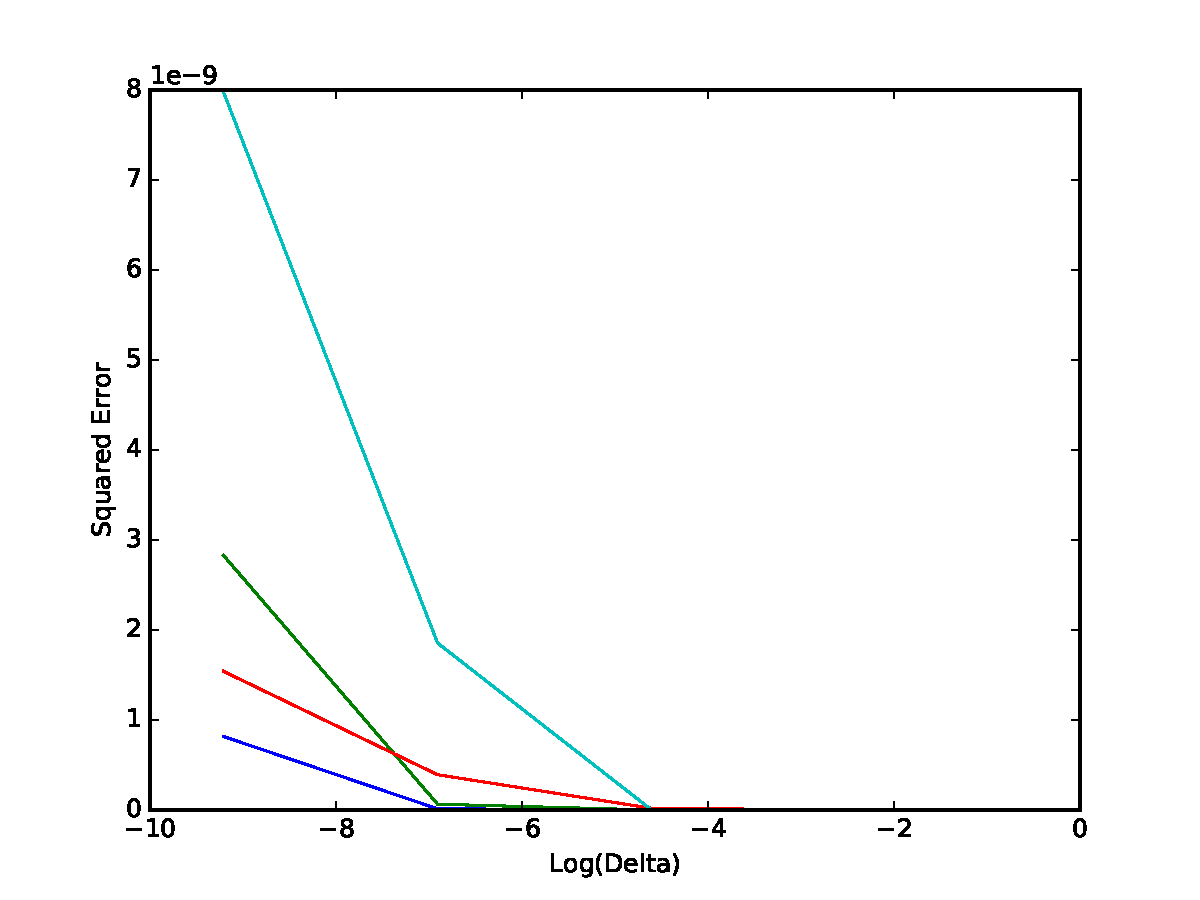
\includegraphics[width=\textwidth]{hw1_1-2b.pdf}
	\caption{Quadratic bowl}
\end{subfigure}
\caption{Squared error of finite difference gradient approximations compared to the exact gradients for differing step sizes.}
\end{figure}

\subsection{Batch vs. Stochastic Gradient Descent on Least Squares}

We now turn to the question of fitting parameter values for a linear model:
$$y = x^T\theta$$
and we want to estimate $\theta$, using a squared loss:
$$J(\theta) = \|X\theta - y\|^2$$
where $X$ is our model matrix. Our goal is to study the relative performance of batch and stochastic gradient descent on this problem. In order to do so, we first derive the batch gradient to be:
$$\nabla_{\theta} J(\theta) = 2X^T(X\theta - y)$$

In the stochastic gradient case, we have the following point-wise gradient:

$$\nabla_{\theta} J_i(\theta; x^{(i)}, y^{(i)}) = 2(x^{(i)T}\theta - y^{(i)}) x^{(i)}$$

We would like to understand how the two algorithms behave under similar conditions. Thus, we explore the accuracy (in terms of $L_2$ distance from the exact solution) as well as the number of evaluations of the pointwise gradient. That is, each iteration of the batch gradient descent counts as $n$ evaluations, where $n$ is the number of data points.

Unfortunately, we found through empirical experiments that SGD simply does not converge to accurate values under typical Robbins-Monro annealing, i.e.:
$$\eta_t = \eta/(\tau_0 + t)^{\kappa}$$
In fact, even when we chose initial $\theta_0$ to be the actual exact solution rounded to the nearest integer, SGD did not yield a reasonable solution. In all of these cases, SGD tended to converge prematurely, even with $\tau_0 = 0$ and $\kappa = 0.5$, the minimum value for the conditions to hold.

Thus, we consider values of $\tau_0, \kappa$ that may lie outside of the guarantees of the Robbins-Monro conditions. Moreover, having SGD use step size annealing while batch GD employs constant step sizes is not an apples-to-apples comparison; consequently, we employ the same step size annealing procedure in both algorithms, augmenting batch GD with such a procedure. We found that a starting step size of $\eta = 10^{-5}$ and convergence criterion of $\epsilon = 10^{-15}$ worked well for most experiments, as shown in the case of the negative Gaussian and quadratic bowl, and keep these fixed. On the other hand, we vary values of $\tau_0, \kappa$ and see how the accuracy and evaluation numbers of the two algorithms compare in these different situations. We also fix the initialization at $\theta_0 = (1, \dots, 1)$ for all experiments.

The results are shown in {\bf Figure 4}. We see that for the same value of $\tau, \kappa$, batch gradient descent uniformly dominates SGD in terms of squared error. Moreover, $\tau$, perhaps as expected, has little effect on the convergence of the algorithms, while $\kappa$ plays a significant role, especially for SGD. When $\kappa$ is too large, SGD terminates prematurely, as shown by part (C), where the number of evaluations of SGD for $\kappa > 10^{-4}$ is negligible compared to the lowest $\kappa$ case. This is directly tied to the accuracy of the SGD algorithm; in all but the smallest values of $\kappa$, the algorithm converges to a substantially inaccurate value. Thus, we see that it is critical to make sure that the annealing of the step sizes is sufficiently slow for the algorithm to converge to the correct value. However, having annealing that is too slow yields an exponential increase in number of evaluations, with negligible gains in squared error (i.e. $\kappa < 10^{-5}$).

\begin{figure}
		\begin{subfigure}[b]{0.8\textwidth}
			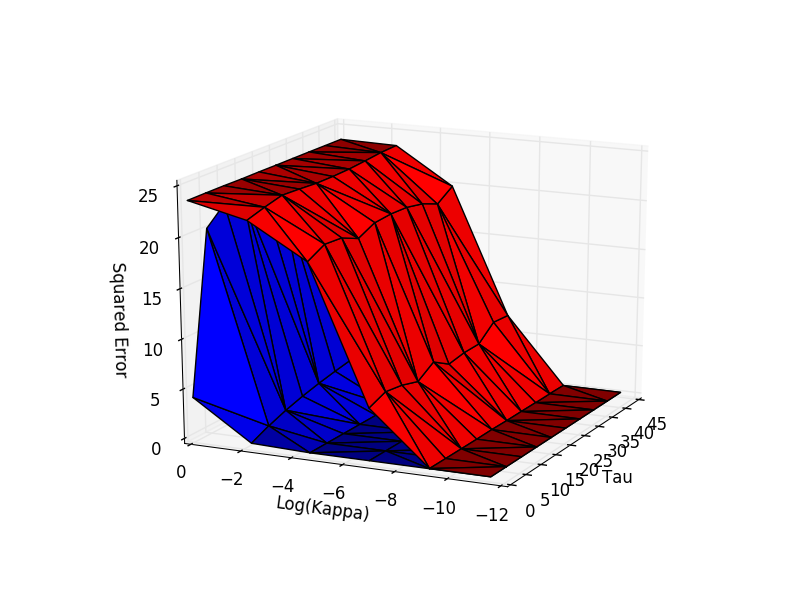
\includegraphics[width=\textwidth]{hw1_1-3_acc_both.png}
			\caption{Squared error for batch (blue) and stochastic (red) gradient descent.}
		\end{subfigure}
			\begin{subfigure}[b]{0.48\textwidth}
				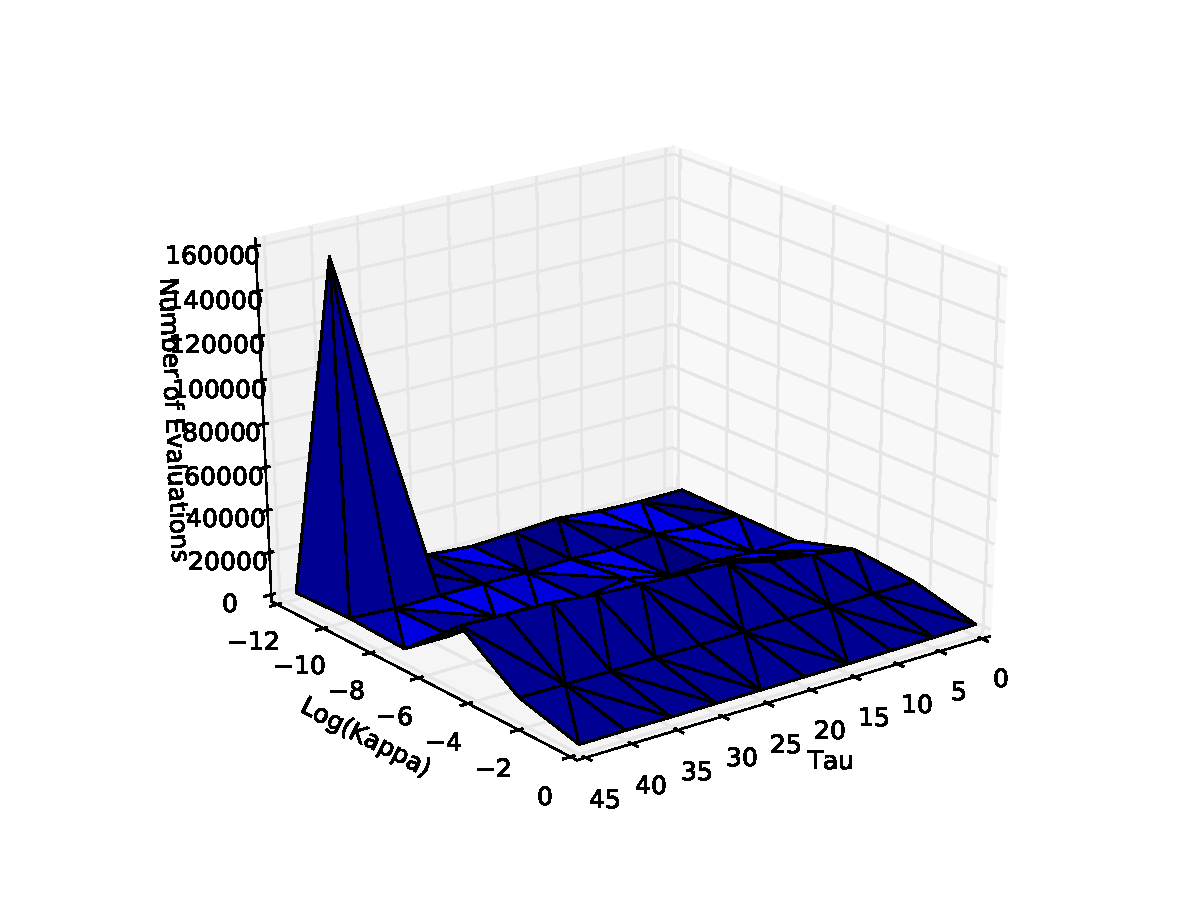
\includegraphics[width=\textwidth]{hw1_1-3_timeGD.pdf}
				\caption{Batch}
			\end{subfigure}
		\begin{subfigure}[b]{0.48\textwidth}
			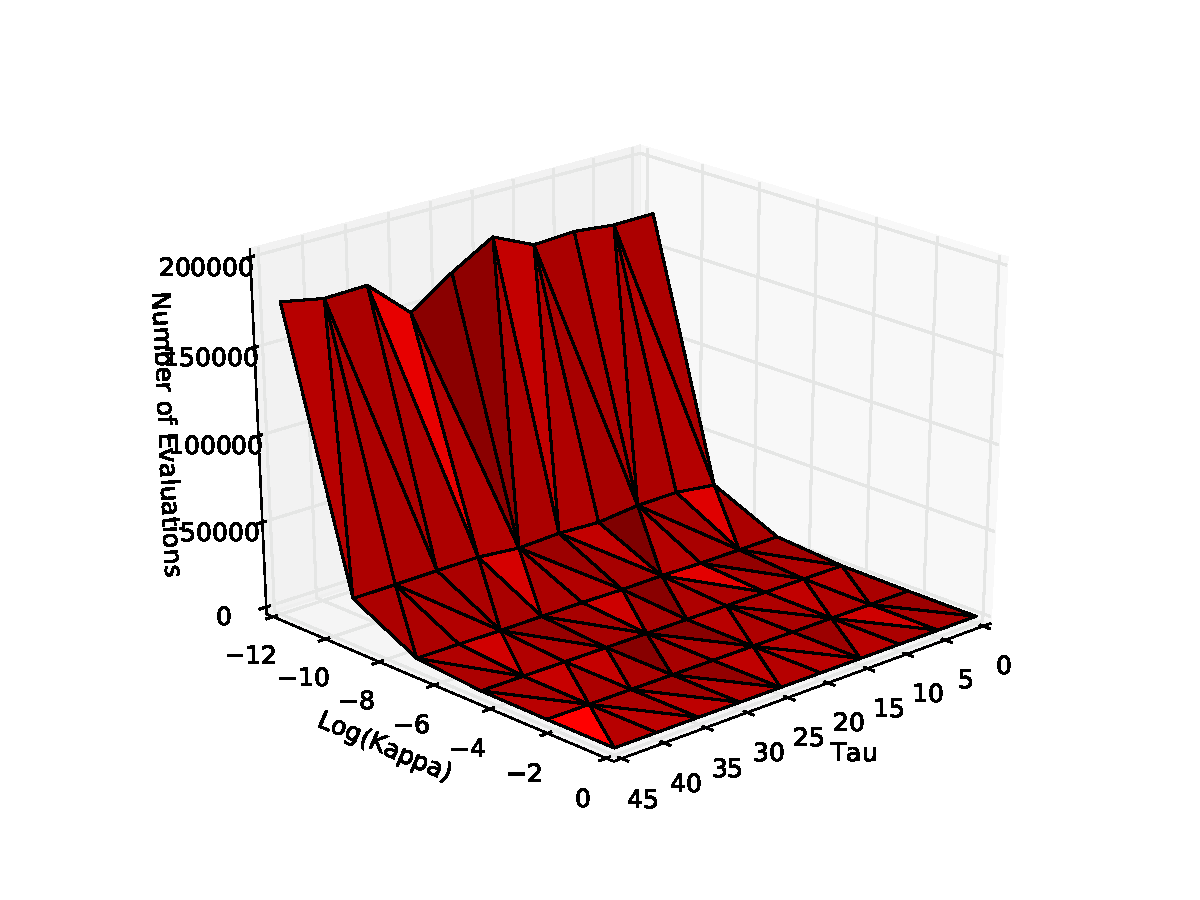
\includegraphics[width=\textwidth]{hw1_1-3_timeSGD.pdf}
			\caption{Stochastic}
		\end{subfigure}			
	\caption{(A) shows the squared error for the two algorithms, while (B) and (C) show number of gradient evaluations for batch and stochastic gradient descent, respectively.}
\end{figure}

\section{Linear Basis Function Regression}

We now turn to the question of linear regression using nonlinear basis functions. We consider the true data model:

$$y(x) = \cos(\pi x) + 1.5 \cos(2\pi x) + \epsilon$$

where $\epsilon$ is small random noise. We start by exploring the suitability of polynomial basis functions for this model, varying the maximum degree of the polynomial terms; namely, we consider the basis:

$$\phi_0(x) = 1, \phi_1(x) = x, \dots, \phi_M(x) = x^M$$

We find, as expected, that lower-order polynomials (i.e. $M = 0, 1$) fail to fit the data well due to their simplicity, whereas polynomials of too high order (i.e. $M = 10$) overfit the data substantially. This is demonstrated in {\bf Figure 5}.

\begin{figure}
	\centering
	\begin{subfigure}[b]{0.24\textwidth}
		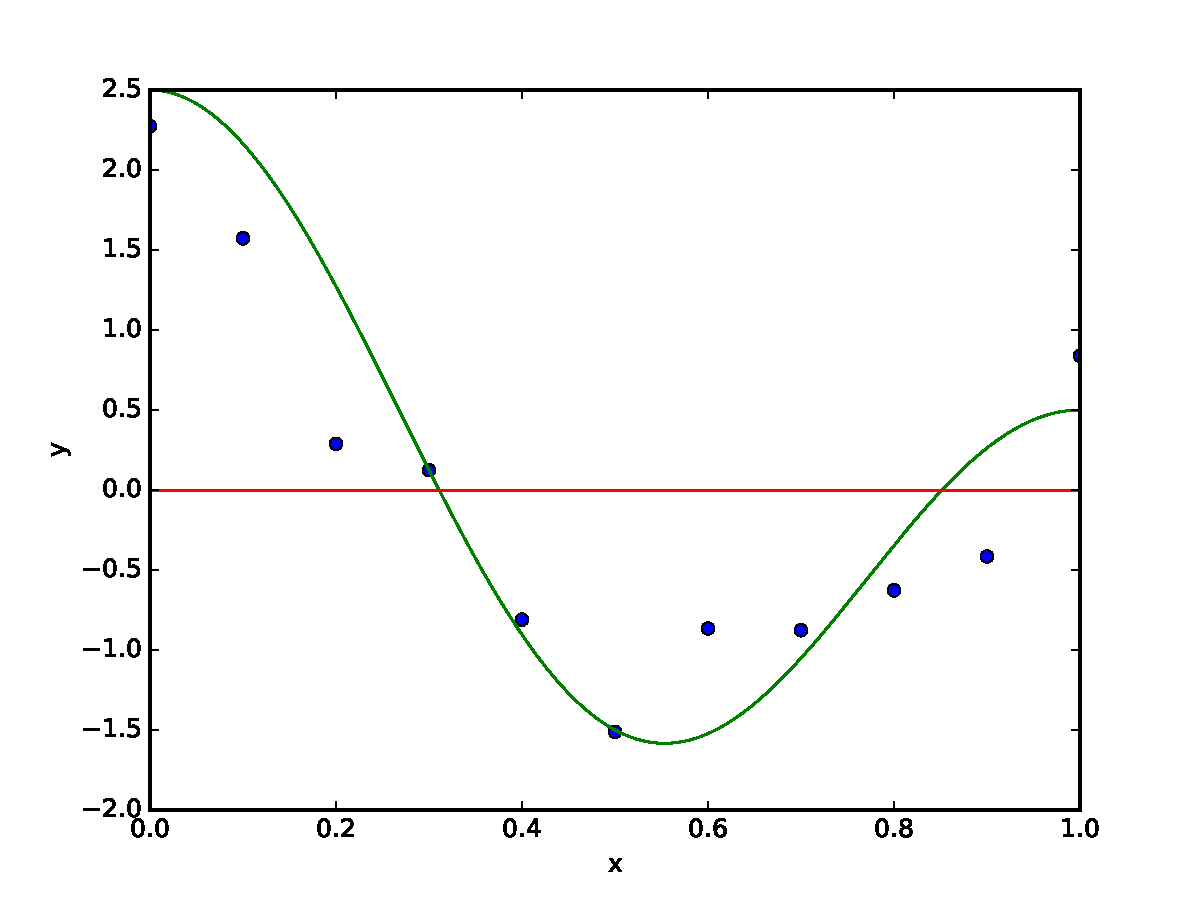
\includegraphics[width=\textwidth]{hw1_2-1_0.pdf}
		\caption{$M=0$}
	\end{subfigure}
	\begin{subfigure}[b]{0.24\textwidth}
		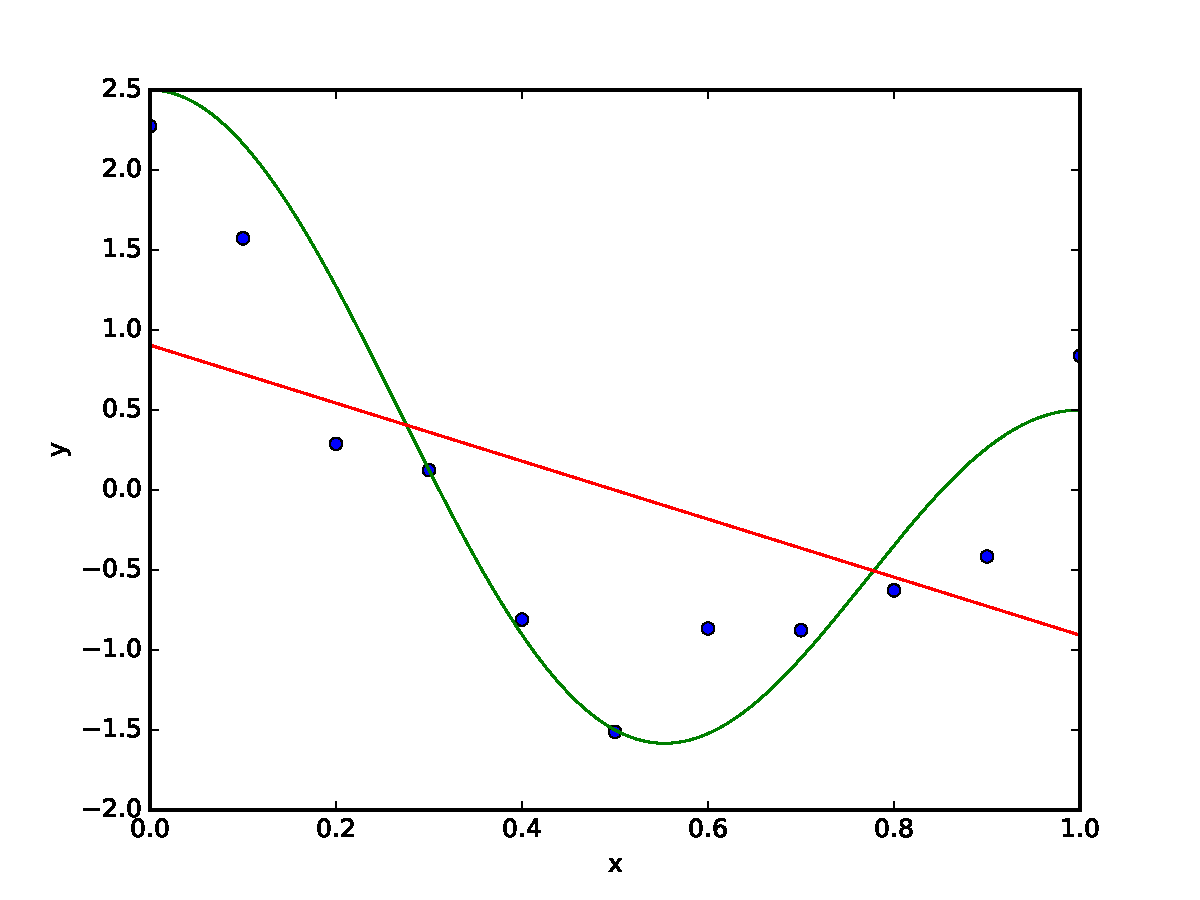
\includegraphics[width=\textwidth]{hw1_2-1_1.pdf}
		\caption{$M=1$}
	\end{subfigure}
	\begin{subfigure}[b]{0.24\textwidth}
		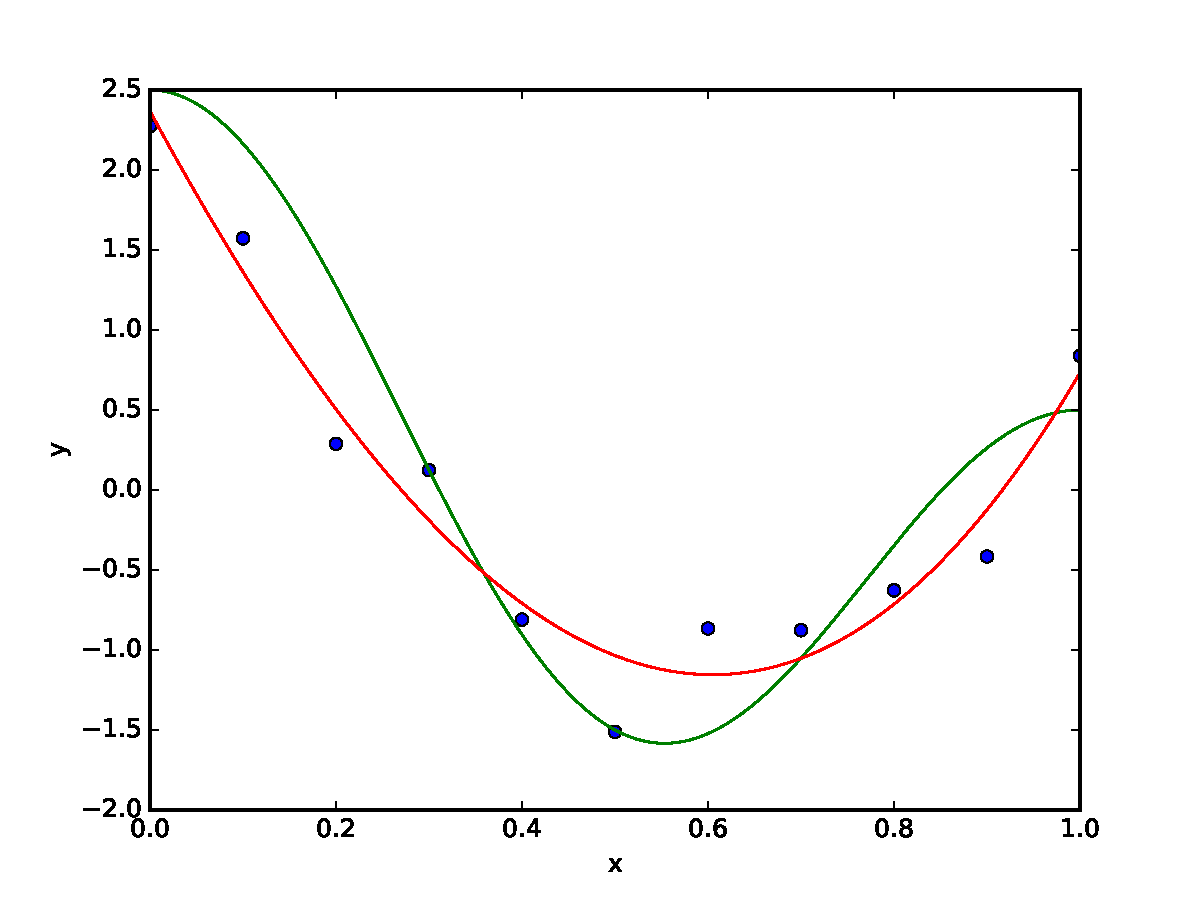
\includegraphics[width=\textwidth]{hw1_2-1_3.pdf}
		\caption{$M=3$}
	\end{subfigure}
	\begin{subfigure}[b]{0.24\textwidth}
		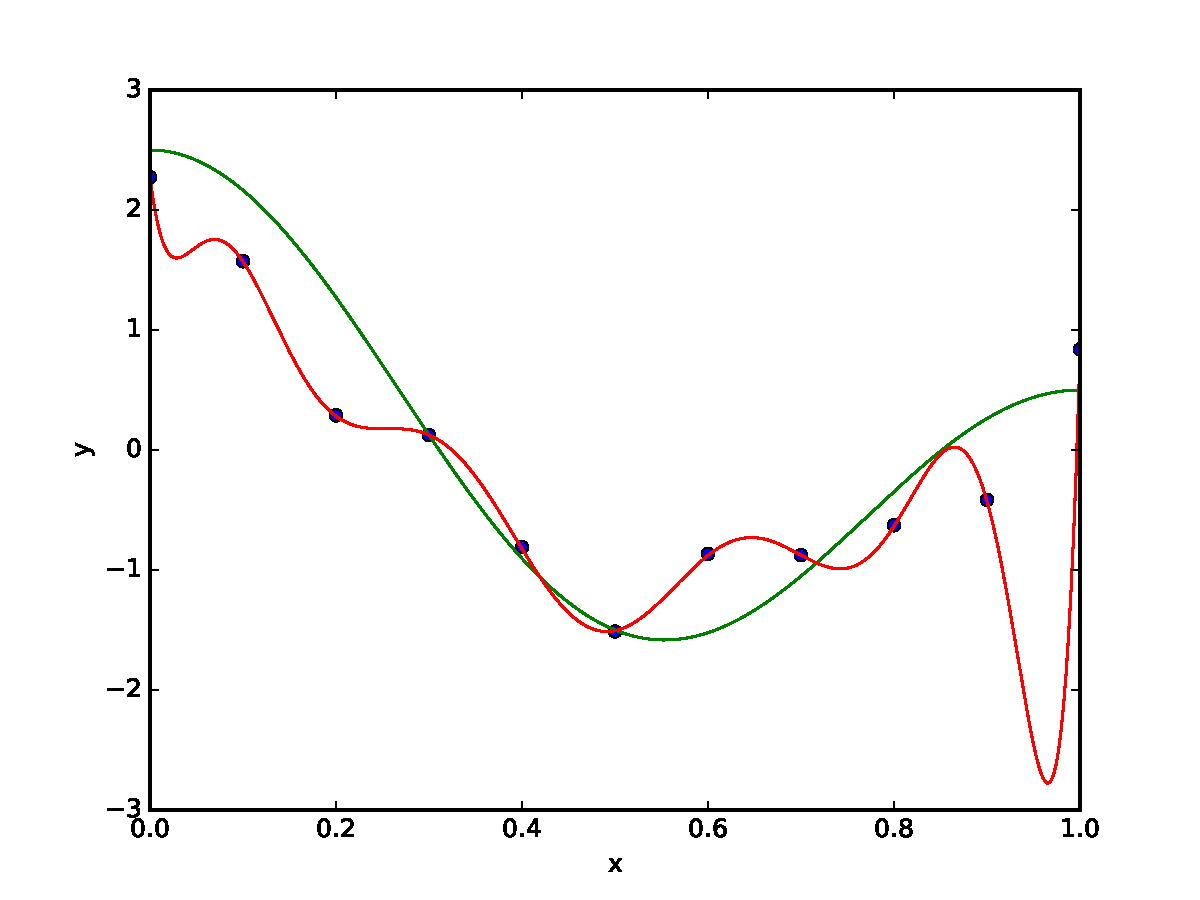
\includegraphics[width=\textwidth]{hw1_2-1_10.pdf}
		\caption{$M=10$}
	\end{subfigure}
	\caption{Polynomial fits to the cosine model, where the green line is the true model and the red line is the polynomial fit of degree $M$.}
\end{figure}

We define the SSE of the dataset and hypothesis as follows. The design matrix is given by:

$$\Phi \equiv \begin{pmatrix} \phi_0(x_1) & \phi_1(x_1) & \cdots & \phi_M(x_1) \\ \vdots & \vdots &  & \vdots \\ \phi_0(x_n) & \phi_1(x_n) & \cdots & \phi_M(x_n)\end{pmatrix}$$

where $\phi_i$ is the $i^{th}$ polynomial basis function, i.e. $\phi_i(x_j) = x_j^i$. Then the SSE for fixed weights $w = (w_0, w_1, \dots, w_M)$ is given by:
$$SSE(w) = \|\Phi w - y\|^2 = \sum_{i=1}^n (\Phi_{i\cdot}w - y)^2$$
in which $\Phi_{i\cdot}$ indicates the $i^{th}$ row of the design matrix. We can then easily derive the derivative of the squared error loss as in linear regression, which yields:

$$\nabla_w SSE(w) = 2 \Phi^T(\Phi w - y)$$

\section{Ridge Regression}

\section{Sparsity and LASSO}

\end{document}


